% !TEX encoding = ISO-8859-16
\section{Introduction}

The mass transportation problem corresponds to the computation of an optimal warping to map (i.e. push-forward) a given input probability measure $\mu_0$ to a second probability measure $\mu_1$. The optimality corresponds to minimizing a cost (the so-called Wasserstein distance) associated to the warping, which measures the effort needed to perform the corresponding motion. Informally, the effort is expressed as the cost it would require to move a pile of sand representing $\mu_0$ toward a hole made of $\mu_1$, by summing the cost (typically a squared distance) for each particle of sand to reach its destination in the hole (see Fig.~\ref{fig:monge}).  We refer to~\cite{Villani03} for a review of the mathematical foundations of optimal transport. 

As a byproduct of the computation of this optimal transport, it is possible to define a geodesic $\mu_t$, for $t \in [0, 1]$ interpolating between the two input measures. This corresponds to the so-called displacement interpolation introduced by McCann~\cite{mccann1997convexity}. Such an interpolation has several  applications ranging from the analysis of PDEs to computer graphics, which we review below. Moreover, as introduced in~\cite{Carlier_wasserstein_barycenter}, this interpolation between two densities can be extended to an arbitrary number of measures by defining a barycenter according to the transportation distance. However, a major bottleneck is the computational complexity of computing the optimal transport, geodesics and barycenters in arbitrary dimension.  In this paper, we address these issues by leveraging the fact that these problems are easy to solve for 1-D distributions. We propose alternative definitions of barycenters using two frameworks based on 1-D projections of the measures. We describe the associated fast computational schemes, and show some applications in image processing (color transfer) and computer graphics (texture mixing).


% The mass transportation problem leads to an interpolation $\mu_t$ ($t \in [0, 1]$), called \textit{displacement interpolation}, that consists  in moving the probability measure $\mu_0$ partway toward $\mu_1$. This has shown to have a wide range of applications, from computer graphics~\cite{Bonneel-displacement,Rabin_ssvm11,matusik2005texture} to image processing~\cite{pitie2005n,haker2004}, due to the characteristic advection produced during the interpolation. While this interpolation can be very efficiently performed in one dimension, extending it to multiple dimensions is much more challenging and leads to computationally expensive solutions. In addition, further extending  the approach to an interpolation between more than two probability measures currently remains untractable. In this paper, we address both scalability and multi-marginal mass transportation through an approximate framework based on 1d projections. We present both a fast Eulerian approach and a more general Lagrangian approach, and analyze some properties they share.

\vspace{0.3cm}
\begin{figure}[!t]
\begin{center}
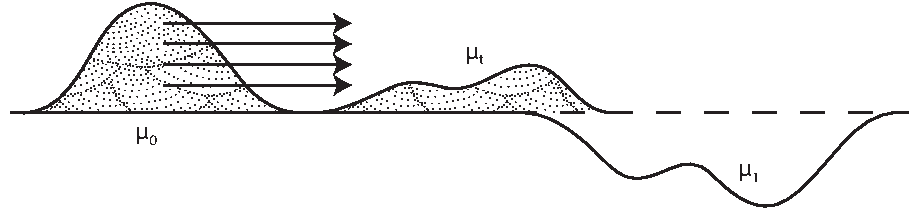
\includegraphics[width=\linewidth]{img/monge.pdf}
\end{center}
\caption{The mass transportation problem consists in optimally moving a probability measure $\mu_0$ represented by a pile of sand, toward a probability measure $\mu_1$ making a hole. At an intermediate time $t \in [0,1]$, an interpolated probability measure $\mu_t$, the \textit{displacement interpolation}, is obtained. A \textit{Wasserstein barycenter} generalizes this notion by considering more than $2$ probability measures.}
\label{fig:monge}
\end{figure}


%%%%%%%%%%%%%%%%%%%%%%%%%%%%%%%%%%%%%%%
\subsection{Previous work}

%%%
\paragraph{Computational Optimal transport.}

There is a vast literature on the numerical computation and approximation of the optimal transport plan. For discrete measures ({i.e.} sums of Dir\-acs), it boils down to the solution of a linear program, as initiated by Kantorovitch~\cite{Kantorovich42} which laid the modern foundations of transportation theory. There exist dedicated combinatorial optimization methods, such as the auction algorithm~\cite{Bertsekas1988} and the Hungarian algorithm~\cite{Kuhn-hungarian}. The $L^2$ optimal transport map is the solution of the celebrated Monge-Amp\`ere non-linear PDE. A variety of methods have been proposed to approximate numerically the solution to this equation, see for instance~\cite{Benamou2012} and references therein. 

% The optimization re\-qui\-red to compute the \textit{transport plan} -- the map that describes the motion of the probability measures -- can be performed in several ways. For instance, Bonneel et al. used a linear program with radial basis functions~\cite{Bonneel-displacement}. Benamou and Brenier exploited a fluid dynamic interpretation~\shortcite{Benamou2000}  which requires solving for a space-time Laplace equation, that Papadakis et al. efficiently performed via proximal splitting~\cite{FPapPeyOud13}. Haker et al. used Brenier's polar factorization to build a curl-free velocity field solving the transportation problem~\cite{haker2004}.  M�rigot proposed a multiscale geometric method based on power diagrams~\cite{Merigot2011} by computing the transport plan between diracs and a smooth density. These approaches however remain complex, and limited to the interpolation between two probability measures. 


%%%
\paragraph{Wasserstein geodesics. }

The Wasserstein geodesic (i.e. a minimizing length path interpolating between two measures) is easily computed by linearly interpolating between the identity and the optimal transport. It is thus a trivial by-product of the computation of the optimal map. Let us however notice that the landmark paper of Benamou and Brenier~\cite{Benamou2000} proposes to actually proceed the other way around, i.e., to compute the geodesic as the solution of a convex optimization problem. The drawback of this approach is that it requires the addition of an extra dimension (time parameterizing the geodesic), but it allows the computation of an accurate approximation of the geodesic on a fixed discretization grid. This algorithm has recently been revisited using proximal splitting optimization schemes~\cite{FPapPeyOud13} ; we make use of this approach to compare the Wasserstein geodesics with the one obtained through our methods. 

%%%
\paragraph{Wasserstein barycenters. }

Wasserstein barycenters generalize the notion of geodesic interpolation from two to an arbitrary number of measures. The mathematical foundation for the formulation of these barycenters (i.e. existence, uniqueness and linear programming formulation) is detailed in~\cite{Carlier_wasserstein_barycenter}. These barycenters have found application, for instance, in statistical estimation~\cite{BigotBarycenter}. They enjoy an almost closed form expression in the case of Gaussian measures. This property is used in~\cite{peyre2013Gaussians} to perform texture mixing of Gaussian texture models. 

Cuturi and Doucet propose in~\cite{CuturiBarycenter} a numerical scheme to approximate the Wasserstein barycenter on an Eulerian grid. They smooth the Wasserstein distance using an entropic penalization, allowing them to perform a gradient descent. To reduce the numerical complexity of the barycenter computation, Rabin et al.~\cite{Rabin_ssvm11} introduce a different variational problem that sums the Wasserstein distances of 1-D projections of the input measures. Our method generalizes the iterative 1-D histogram matching used in~\shortcite{pitie2005n} to alter color palettes. Our work builds on the initial construction of  Rabin et al.~\cite{Rabin_ssvm11}. We propose a more formal exposition of this method and its main properties, and also present an alternative formulation based on the Radon transform. 



%%%
\paragraph{Applications in imaging. }

There are numerous applications of mass transportation in image processing, computer vision and computer graphics. The Wasserstein distance leads to state-of-the-art results for several image retrieval problems, see for instance~\cite{Rubner1998} for an early work on this topic. The optimal transport plan has been used for color transfer in images~\cite{pitie2005n} and for meshing in computer graphics~\cite{digne-reconstruction}.  Displacement interpolation has been employed for image warping and registration~\cite{haker2004,Merigot2011}, to remove flickering in old movies~\cite{Delon-midway} and in computer graphics to perform manipulations on textures~\cite{matusik2005texture} and to interpolate reflectance for 3-D rendering~\cite{Bonneel-displacement}. The Wasserstein barycenter of Gaussian distributions has found applications for texture synthesis and mixing, using either non-parametric density estimations~\cite{Rabin_ssvm11} and Gaussian density estimation~\cite{peyre2013Gaussians}.


%%%%%%%%%%%%%%%%%%%%%%%%%%%%%%%%%%%%%%%%%%%%%%%%%%%%%%%%%%%%%%%%
\subsection{Contributions}

In this paper, we introduce two efficient methods to approximate the Wasserstein barycenter of an arbitrary number of measures based on 1-D projections. The first approach, that we call ``Radon barycenter'', computes 1-D barycenters of Radon projections of the input measures, and defines the resulting barycenter as a back-projection of these 1-D barycenters. This method leads to a fast numerical scheme for an Eulerian discretization of the measures (i.e. based on histograms on a regular lattice), using a discrete Radon transform.  The second approach, that we call ``sliced barycenter'', is defined as the solution of an optimization problem which integrates the distances of all the Radon projections. A Lagrangian discretization (i.e. using point clouds with freely moving positions) is well adapted to the numerical resolution of a non-convex re-formulation of this optimization problem. 

We demonstrate properties of these two barycenters, analyze their relationship and show how they compare in practice. We show that both approximations solve a similar variational problem that only differs in the lack of surjectivity of the Radon transform. We also prove that both barycenters exhibit similar translational and scaling properties as the exact Wasserstein barycenter at a fraction of its computational cost. We compare our approximation with  the exact barycenter of two probability measures using a state of the art method~\cite{FPapPeyOud13}. We exemplify typical usages of these two complementary approaches to solve a problem of color harmonization in image processing, and a problem of texture mixing in computer graphics. 

The code to reproduce the figure of this article is available online\footnote{\url{https://github.com/gpeyre/2014-JMIV-SlicedTransport}}.


%%%%%%%%%%%%%%%%%%%%%%%%%%%%%%%%%%%%%%%%%%%%%%%%%%%%%%%%%%%%%%%%
\subsection{Notations}

We denote $\SS^{d-1}$ the unit sphere in $\RR^d$, and we define $\Om^d = \RR \times \SS^{d-1}$. 
We denote $\d \th$ the uniform measure on the sphere, which is normalized to satisfy $\int_{\Sph} \d\th=1$. We write $\Cont{X}$ the space of continuous functions on $X$ tending to 0 at infinity, where in the following $X$ is either $\RR^d$ or $\Om^d$. It is a Banach space with respect to the norm 
\eq{
	\foralls f \in \Cont{X}, \quad \normi{f}=\umax{x \in X} |f(x)|.
} 
We denote as $\Mm(X)$ the Radon measures on $X$, which is the space of finite Borel measures on $X$, and can also be represented as the dual of $\Cont{X}$, i.e., it is the space of continuous linear forms on $\Cont{X}$. We write 
\eq{
	\foralls (\mu,g) \in \Mm(X) \times \Cont{X}, \quad 
		\int_X g(x) \d \mu(x) \in \RR
}
the duality pairing between these spaces, which evaluates at $g$ the linear form defined by $\mu$. $\Mm(X)$ is a Banach space with respect to the dual norm, which is the so-called total variation norm, $\foralls \mu \in \Mm(X)$
\eql{\label{eq-tv-norm}
	\norm{\mu}_{\text{TV}} = \max \enscond{ \int_X g(x) \d \mu(x) }{ g \in \Cont{X}, \; \normi{g} \leq 1 }.
}
In the following, the convex cone of positive Radon measures is written 
\eq{
	\Mm^+(X) = \enscond{ \mu }{ \foralls f \in \Cont{\RR^d}, f \geq 0, \: \int f \d\mu \geq 0 }.
} 

We denote as $\sharp$ the push-forward operator, which, for any measurable map $M : X \rightarrow Y$ defines a linear operator $M\sharp : \Mm(X) \rightarrow \Mm(Y)$ as, for any $\mu \in \Mm(X)$  
\eq{
	\foralls g \in \Cont{Y}, \quad
	\int_Y g(y) \d(M \sharp \mu)(y) = 
	\int_X g(M(x)) \d\mu(x).
}
If $\d\mu(x) = \rho(x)\d x$ has a density $\rho$ with respect to some measure $\d x$ (e.g., the Lebesgue measure on $\RR^d$), and if $M$ is a $C^1$ diffeomorphism, then one has
\eql{\label{eq-pushfwd-density}
	\d (M \sharp \mu)(y) = (\rho \circ M^{-1})(y) |\det(\partial M^{-1}(y))| \d y.
}

Using the disintegration theorem (see for instance~\cite{DellacherieBook}), one can slice a measure $\nu \in \Mm(\Om^d)$ into its conditional measures with respect to the uniform measure on $\SS^{d-1}$ to obtain a measure $\nu^\th \in \Mm(\RR)$ for almost all $\th \in \SS^{d-1}$ outside a Borel set of zero measure, which satisfies, $\foralls g \in \Cont{\Om^d}$
\eql{\label{eq-desintegration}
	\int_{\Om^d} g(t,\th) \d \nu(t,\th) = 
	\int_{\SS^{d-1}} \pa{ \int_\RR g(t,\th) \d\nu^\th(t)  } \d \th,
}
and such that for any Borel set $A \subset \RR$, $\th \in \SS^{d-1} \mapsto \nu^\th(A) \in \RR$ is a Borel map. 

The convex set of normalized positive probability measures is $\Mm_1^+(\RR^d) \subset \Mm^+(\RR^d)$, which are measures $\mu \in \Mm^+(\RR^d)$ which satisfy $\mu(\RR^d)=1$.
We also denote $\bar\Mm_1^+(\Om^d)$ the set of positive probability measures having normalized conditional mesures along the $t$ variable, i.e.,
\eq{
	\bar\Mm_1^+(\Om^d) = \enscond{ \nu \in \Mm_1^+(\Om^d) }{ \foralls \th \in \SS^{d-1}, \quad \nu^\th(\RR) = 1 }
}
where $\nu^\th \in \Mm_1^+( \RR )$ is the conditional measure defined according to the disintegration formula~\eqref{eq-desintegration}. 

We denote as $\de_x \in \Mm_1^+(\RR^d)$ the Dirac measure at $x \in \RR^d$, i.e. 
\eq{
	\foralls f \in \Cont{\RR^d}, \quad
		\int_{\RR^d} f(y) \d (\de_x)(y) = f(x).  
}

We write $\Dd(X)$ the space of $\Cc^\infty(X)$ functions with compact support, and $\Dd^*(X)$ its dual, which is the space of distributions.  

% We write $H^s(X)$ the Sobolev space of order $s$, which is the set of $f \in \Dd^*(X)$ such that $f^{(s)} \in \Ldeux(X)$ (possibly interpreted as a fractional derivative if $s$ is not integer). One has $\Mm(X) \subset H^s(X) \subset \Dd^*(X)$ for any $s<-d/2$ \todo{negative $d/2$? sure ?}.


The Fourier transform of $f \in \Lun(\RR^d)$ is defined as
\eq{
	\foralls \om \in \RR^d, \quad \hat f(\om) = \int_{\RR^d} f(x) e^{-\imath \dotp{\om}{x}} \d x,
}
and the Fourier transform of a measure $\mu \in \Mm(\RR^d)$ as
\eq{
	\foralls \om \in \RR^d, \quad \hat \mu(\om) = \int_{\RR^d} e^{-\imath \dotp{\om}{x}} \d \mu(x).
}

Given a finite index set $I$, we define the simplex set of weights as 
\eql{\label{eq-defn-simplex}
	\La_I = \enscond{ \la = (\la_i)_{i \in I} \in \RR^I }{ \foralls i \in I, \: \la_i \geq 0, \; \sum_{i \in I} \la_i = 1 }
}
where the notation $\RR^I$ corresponds to the set of vectors indexed by $I$. 
%For $\la \in \La_I$, we also define the mapping
%\eq{ 
%	\be_\la : x = (x_i)_{i \in I} \in  (\RR^d)^I \mapsto \sum_{i \in I} \la_i x_i \in \RR^d.
%}

We define the following translation and scaling operators, for all $(s,u) \in \RR^{+,*} \times \RR^d$, 
\begin{align*}
		\foralls x \in \RR^d, \quad
			\phi_{s,u}(x) &= s x + u \in \RR^d, \\ 
		\foralls (t,\th) \in \Om^d, \quad
			\psi_{s,u}(t, \th) &= (st+\dotp{u}{\th}, \th) \in \Om^d.
\end{align*}
We denote $\Oo(\RR^d)$ the orthogonal group of $\RR^d$, i.e. $\Phi : \RR^d \mapsto \RR^d$ is an invertible linear map with $\Phi^* = \Phi^{-1}$ the adjoint operator. For all $\Phi \in \Oo(\RR^d)$ we denote  
\eq{
	\tilde \Phi : (t,\th) \in \Om^d \mapsto (t,\Phi^* \th) \in \Om^d.
}
A measure $\mu$ is said to be radial (denoted $\mu \in \Rad(\RR^d)$) if $\Phi \sharp \mu = \mu$ for all rotation $\Phi \in \Oo(\RR^d)$. 
It is said to be centrally symmetric (denoted $\mu \in \Cent(\RR^d)$) if $S \sharp \mu = \mu$ for the central symmetry $S \in \Oo(\RR^d)$ such that $S = -\Id_{\RR^d}$. 
